\documentclass[11pt]{article}

% ============================================================
%  Packages
% ============================================================
\usepackage[margin=1in,top=0.95in,bottom=1in]{geometry}
\usepackage{amsmath}
\usepackage{amssymb}
\usepackage{booktabs}
\usepackage{array}
\usepackage[skip=6pt,font=small]{caption}
\usepackage{enumitem}
\usepackage{titlesec}
\usepackage{xcolor}
\usepackage[most]{tcolorbox}
\usepackage{graphicx}
\usepackage{microtype}
\usepackage[hidelinks]{hyperref}

\graphicspath{{figures/}{./}}

% ============================================================
%  Color tokens: RAND purple accent, matching the briefing deck
% ============================================================
\definecolor{randpurple}{HTML}{761DDB}
\definecolor{purpledk}{HTML}{4E1291}
\definecolor{purplebg}{HTML}{F5EFFD}
\definecolor{ink}{HTML}{1C1C1E}
\definecolor{rulegray}{HTML}{D9D5D2}
\definecolor{mutegray}{HTML}{6E6660}
\definecolor{graybg}{HTML}{F4F3F1}
\definecolor{graydk}{HTML}{4A4A4C}
\definecolor{warnred}{HTML}{C00000}

\color{ink}

% ============================================================
%  Typography
% ============================================================
\setlength{\parindent}{0pt}
\setlength{\parskip}{0.52em}
\setlist{itemsep=3pt, topsep=3pt, parsep=0pt}
\linespread{1.05}

\titleformat{\section}
  {\large\bfseries\color{purpledk}}
  {\thesection.\ }{0.4em}{}
  [{\vspace{2pt}\color{randpurple}\titlerule[0.9pt]}]
\titlespacing*{\section}{0pt}{17pt}{8pt}

\titleformat{\subsection}
  {\normalsize\bfseries\color{ink}}
  {\thesubsection\ }{0.4em}{}
\titlespacing*{\subsection}{0pt}{12pt}{3pt}

\setcounter{secnumdepth}{2}

% Float placement: let figures share a page with text
\renewcommand{\topfraction}{0.88}
\renewcommand{\bottomfraction}{0.70}
\renewcommand{\textfraction}{0.10}
\renewcommand{\floatpagefraction}{0.80}

% ============================================================
%  Boxes
% ============================================================
\newtcolorbox{keybox}[1][]{
  enhanced,
  colframe=randpurple,
  colback=purplebg,
  boxrule=0.9pt,
  sharp corners,
  left=11pt, right=11pt, top=9pt, bottom=9pt,
  fonttitle=\bfseries\footnotesize,
  coltitle=white,
  colbacktitle=randpurple,
  title={\MakeUppercase{Key concept}\;\textbullet\;#1},
  attach boxed title to top left={xshift=0pt, yshift=0pt},
  boxed title style={sharp corners, boxrule=0pt},
  before skip=10pt, after skip=10pt,
  breakable,
}

\newtcolorbox{workbox}[1][]{
  colframe=graydk,
  colback=graybg,
  boxrule=0.6pt,
  sharp corners,
  left=11pt, right=11pt, top=9pt, bottom=9pt,
  fonttitle=\bfseries\footnotesize,
  coltitle=white,
  title={\MakeUppercase{Worked example}\;\textbullet\;#1},
  before skip=10pt, after skip=10pt,
  breakable,
}

\newtcolorbox{promptbox}[1][]{
  colframe=mutegray,
  colback=white,
  boxrule=0.5pt,
  sharp corners,
  left=10pt, right=10pt, top=8pt, bottom=8pt,
  fontupper=\ttfamily\footnotesize,
  fonttitle=\bfseries\footnotesize\color{white},
  coltitle=white,
  colbacktitle=mutegray,
  title={#1},
  before skip=9pt, after skip=9pt,
  breakable,
}

\newcommand{\term}[1]{\textbf{\color{purpledk}#1}}

% ============================================================
\begin{document}

% Title block
\begin{flushleft}
{\color{randpurple}\rule{\linewidth}{1.6pt}}\\[10pt]
{\LARGE\bfseries\color{ink} Does an AI Have a Money Personality?}\\[6pt]
{\Large\color{ink} An Experiment in Machine Behavioral Economics}\\[9pt]
{\large\color{purpledk} A teaching paper for undergraduate economics students}\\[11pt]
{\color{rulegray}\rule{\linewidth}{0.8pt}}\\[7pt]
{\small\color{ink}\textbf{John Blakeslee}, RAND School of Public Policy \hfill
 AI Sprint Practicum \quad$\cdot$\quad September 2026}\\[3pt]
{\color{randpurple}\rule{\linewidth}{1.6pt}}
\end{flushleft}

\vspace{6pt}

\begin{tcolorbox}[
  colframe=randpurple, colback=purplebg, boxrule=0.6pt, sharp corners,
  left=12pt, right=12pt, top=9pt, bottom=9pt, before skip=2pt, after skip=13pt]
{\small\itshape\color{ink} Who this is for: a student who has taken intermediate
microeconomics and has never studied artificial intelligence. You need to know what a utility
function is, what an expected value is, and that some people are risk averse. You need to know
nothing at all about how an AI model is built. Every AI idea in this paper gets a boxed
explanation the first time it appears, and every economics idea gets a boxed refresher.}
\end{tcolorbox}

% ============================================================
\section*{Abstract}
\addcontentsline{toc}{section}{Abstract}
\small

Economists infer what people want from what they choose. This paper applies that method to
language models, the systems behind AI assistants, and asks a question the field has mostly
skipped: at which point in a model's construction does its handling of money and risk appear?
We put 1{,}680 identical money questions to eleven versions of four AI systems, including four
published snapshots taken at successive stages of one model's training. Five results follow.
Freshly pre-trained models answer with total confidence and pick the larger of two sure payments
barely more often than a coin flip, between 55.5 and 63.9 percent of the time, so their answers
are not preferences in any usable sense. The measurable behavior appears at the first and
simplest stage of assistant training, supervised fine-tuning, and the two later
human-feedback stages move nothing we can detect. The same finished model behaves like two
different subjects depending on whether the question arrives as a chat message or as raw text to
complete, and which format works reverses across model families. Rewording a bet so its downside
reads as a loss changes gambling by $-30.2$ points in one system and $+62.6$ in another, so the
famous framing effect is a property of a particular training recipe rather than of the
technology. Finally, instructing a model in plain language to maximize expected value raises
compliance from about 45 to 54 percent, close to indifference, while the same instruction is
followed almost perfectly on questions requiring no arithmetic. We treat the interpretation of
the second result as a lesson in identification: the data cannot separate training that created
these dispositions from training that made a latent disposition readable, and we show why the
policy conclusion holds under either story.

\normalsize
\vspace{4pt}

% ============================================================
\section{The question, and why an economist can answer it}

Start with a question you can answer yourself before reading any further.

\begin{promptbox}[The cover question]
You must pick one of two payment options.\\
Option A: receive \$86 for certain\\
Option B: a 43\% chance to receive \$210, otherwise nothing\\
Pick the option you prefer.
\end{promptbox}

Most people take a few seconds with that one. The gamble is worth more on average, and it leaves
you with nothing more than half the time. Which option you pick says something about how you
handle risk, and economists have been learning about people by asking questions of exactly this
shape since the 1970s.

We asked AI models thousands of such questions. Then, for one model, we asked the same questions
at four separate points in its construction and watched what changed. The headline of the paper
is that almost everything about how this model handles money arrives at a single manufacturing
step, and that step is the first and least glamorous one.

Before any of that can mean anything, two vocabularies have to be in place. The first is the
economics, which you have seen. The second is the AI, which we assume you have not.

\subsection{The economics you already have}

\begin{keybox}[Revealed preference]
The founding move of choice theory. Rather than ask a person what they value, watch what they
choose when the options are priced, and infer the preference that would rationalize the choices.
The method needs no interview, no self-report, and no cooperation from the subject. It needs only
that the subject makes choices and that the analyst controls the menu. That last condition is
what makes the method portable to a machine: an AI model will not tell you its utility function,
and would have no reliable access to it if asked, but it will pick A or B.
\end{keybox}

\begin{keybox}[Expected value]
The average payoff of a gamble, weighting each outcome by its probability. For a lottery paying
$h$ with probability $p$ and nothing otherwise, $\mathrm{EV} = p \cdot h$. In the cover question,
$\mathrm{EV} = 0.43 \times \$210 = \$90.30$, against a sure \$86. The gamble is worth \$4.30 more
on average. A decision-maker who cared only about the average would take the gamble.
\end{keybox}

\begin{keybox}[Risk aversion]
Most people do not care only about the average. Offered a fair coin flip between \$0 and \$100
against a sure \$50, the majority take the \$50, which means the certainty is worth something to
them beyond the money. In the standard treatment this is curvature in the utility function:
$u$ is concave, so $u(\$50) > 0.5\,u(\$0) + 0.5\,u(\$100)$. A risk-averse person can decline the
cover gamble even though it pays more on average, and nothing is wrong with them for doing so.
\end{keybox}

\begin{workbox}[Pricing the cover gamble, and why we need a second kind of question]
Take the cover question apart. The certain option pays \$86. The gamble pays $0.43 \times \$210 =
\$90.30$ on average. So:

\begin{itemize}
  \item A \term{risk-neutral} agent, who maximizes expected value and nothing else, takes the
  gamble. \$90.30 beats \$86.
  \item A \term{risk-averse} agent may decline. The gamble's \$4.30 premium may not compensate
  for the 57 percent chance of walking away with nothing.
\end{itemize}

Both answers are defensible. That is the problem. If a subject picks the sure \$86, we cannot
tell whether we are watching a coherent risk-averse decision-maker or a subject who is not
engaging with the question at all. A single answer to a single interesting question carries no
information about whether the subject is paying attention.

So we ask a second kind of question, where only one answer is defensible:

\begin{quote}\ttfamily\footnotesize
Option A: receive \$142 for certain\\
Option B: receive \$179 for certain
\end{quote}

No probability, no risk, no taste involved. \$179 is more money than \$142. Every coherent
preference ordering picks B. We call these the \term{dominant controls}, or informally the free
money questions, and there are 80 of them scattered through the instrument. They function
exactly the way an attention check functions in a survey. A subject who fails them has not
revealed unusual preferences. That subject has revealed that its answers are not about the
money.
\end{workbox}

Hold onto that distinction. It carries the first finding of the paper and it is the cheapest
methodological contribution the project makes.

\subsection{The AI you probably do not have}

\begin{keybox}[What a language model is]
A language model is a function that takes a stretch of text and returns a probability
distribution over what comes next. Give it \texttt{The capital of France is}, and it returns a
list assigning high probability to \texttt{Paris}, lower probability to \texttt{a}, lower still
to \texttt{located}, and so on across a vocabulary of tens of thousands of pieces. That is the
entire mechanism. Everything an AI assistant appears to do is that operation run repeatedly,
each predicted piece appended to the text and fed back in. The model has hundreds of millions to
hundreds of billions of adjustable numbers, called \term{weights}, and training is the process of
setting them.
\end{keybox}

\begin{keybox}[Pre-training]
The first and by far the most expensive training stage. The model is shown an enormous quantity
of text, a large fraction of the public internet plus books and code, and its weights are
adjusted so that it predicts each next piece of text better. That is the whole objective. It is
never told what a helpful answer looks like, never told to follow an instruction, and never
rewarded for being correct. A model in this state is called a \term{base model}: it has read a
huge chunk of the internet and nothing else. Asked a question, it does not answer. It continues
the text, which is a different behavior that sometimes resembles answering.
\end{keybox}

\begin{keybox}[Supervised fine-tuning]
The first stage of turning a base model into an assistant, usually abbreviated SFT. Humans write
or curate a set of example exchanges, each a request paired with a good response, and the model's
weights are adjusted to make those responses more likely. The mechanism is identical to
pre-training, next-piece prediction, and only the data has changed: from whatever was on the
internet to a curated set of demonstrations of being helpful. This stage is comparatively cheap,
comparatively unfashionable, and it is where our headline result lands.
\end{keybox}

\begin{keybox}[Preference training]
The stage that follows. Humans are shown two candidate responses to the same request and asked
which they prefer. Those comparisons are used to push the model toward the responses people
picked. Two implementations dominate: reinforcement learning from human feedback (RLHF), which
trains a separate scoring model and then optimizes against it, and direct preference optimization
(DPO), which skips the scoring model and adjusts the weights directly from the comparisons. The
distinction does not matter for this paper. What matters is that this is the stage where human
judgment enters the weights, and it is therefore the usual suspect whenever a model displays a
recognizably human quirk.
\end{keybox}

The ordering is what makes the study possible. Pre-training, then supervised fine-tuning, then
preference training, then a final polish, and the finished assistant is what the public uses.
Nearly all published work on AI decision-making tests only that finished assistant. Testing the
finished product tells you the behavior exists. It cannot tell you which step installed it,
which is the question an auditor, a procurement officer, or a regulator would actually want
answered.

% ============================================================
\section{How we asked}

\subsection{The instrument}

The full instrument is a grid of 1{,}680 questions. It is built from 40 gambles, generated
procedurally so that none of them is a famous textbook problem the model might have memorized.
Each gamble is rewritten five ways using different wordings, and each wording is shown in both
possible orders so that a model with a bias toward the first option is caught by the design.
Each gamble also appears under three framings, described below. The 80 free money questions sit
inside the same grid.

Only one feature moves at a time. Any change in behavior between two cells traces to the one
feature that differs between them, which is the entire reason for building an instrument this
way rather than writing a few questions by hand.

\begin{keybox}[Framing and reference dependence]
Kahneman and Tversky's central observation is that people evaluate outcomes as gains and losses
measured from a reference point, rather than as final states of wealth, and that losses loom
larger than equivalent gains. The practical consequence is that the same choice, described two
ways, gets two different answers. Standard theory says this should not happen. If two options
leave you in identical final positions, the wording is decoration.

Our instrument tests exactly that. Here is the same gamble under two framings:

\begin{quote}\ttfamily\footnotesize
GAIN: Term A: a 64\% chance to gain \$98 and a 36\% chance to gain nothing\\
\phantom{GAIN: }Term B: a certain gain of \$63

MIXED: You have been given \$63 up front.\\
\phantom{MIXED: }Arrangement A: keep your \$63 with no change\\
\phantom{MIXED: }Arrangement B: a 64\% chance to rise to \$98 (a gain of \$35) and a\\
\phantom{MIXED: Arrangement B: }36\% chance to drop to \$0 (a loss of \$63)
\end{quote}

Final wealth is identical in both. Only the reference point moves, from \$0 to \$63, which turns
part of the gamble's downside into a described loss. The \term{frame gap} is the difference in
how often the model gambles between the two: mixed minus gain, in percentage points. A
frame-invariant decision-maker scores zero.
\end{keybox}

\subsection{Reading the answer}

\begin{keybox}[Why we read the model's internal odds instead of sampling its text]
We never make the model type a reply. Recall that a language model returns a probability
distribution over the next piece of text. At the position where the answer letter belongs, we
read that distribution directly and record the probability it assigns to \texttt{A} against the
probability it assigns to \texttt{B}, normalized to sum to one. That number is our observation:
a probability of choosing the gamble, per question, not a binary choice.

Three advantages follow. First, precision. Sampling text 25 times to estimate a choice frequency
gives a noisy estimate of the same quantity one forward pass gives exactly. Second, cost: one
pass per question instead of 25. Third, and most important for this study, base models cannot be
made to answer a question in a usable format, so any method requiring a parseable typed reply
simply cannot be run on them. Reading the distribution works on every model at every training
stage, which is what makes the stage-by-stage comparison possible at all.

There is also a statistical benefit. These readings are deterministic: the same question always
returns the same numbers. All the randomness in the experiment is randomization we control, in
the wordings, the orders, and the payoff grid, which is what our confidence intervals are
computed over.
\end{keybox}

Since the observations are probabilities rather than yes-or-no choices, the estimation uses the
fractional-response likelihood of Papke and Wooldridge (1996) in place of the usual binary
logit, with everything else in the structural model unchanged. That machinery is described in the
technical companion to this paper and is not needed to follow the results here. The two
quantities that carry the argument require no model at all:

\begin{itemize}
  \item \term{Dominance compliance}: the average probability placed on the strictly larger sure
  amount, across the 80 free money questions. An engaged subject scores near 100. A coin flip
  scores 50.
  \item \term{The frame gap}: how much more often the model gambles under loss wording than
  under gain wording, on bets that are arithmetically identical. Frame invariance scores zero.
\end{itemize}

\subsection{The subjects, and the one that makes the study work}

\begin{keybox}[Open-weight models, and why OLMo's published snapshots matter]
A \term{closed} model such as Claude or GPT is available only through a service. You send text,
you get text back, and the weights stay with the developer. An \term{open-weight} model publishes
the trained numbers themselves, so anyone can download the model and run it on their own
hardware.

Open weights alone are not enough for this study. Most open-weight releases publish two things: a
base model and a finished assistant. Comparing those two tells you that post-training changed the
behavior, without telling you which of the three or four post-training stages did it.

OLMo-2, from the Allen Institute for AI, is the exception and is the reason this project exists in
its current form. It publishes a snapshot of the weights after each stage along one training
path: base, after supervised fine-tuning, after preference training, and the finished assistant.
Four snapshots, one lineage, no branching. Asking identical questions of all four turns a coarse
before-and-after comparison into a stage-level attribution. No frontier developer publishes
anything comparable, which is a fact we return to in Section~9.
\end{keybox}

The full subject list is eleven runs: Qwen2.5-7B and Llama-3.1-8B, each as a base model and as a
finished assistant, plus the four OLMo-2 stages, plus every finished assistant run a second time
under an alternative question format. Claude Haiku, a closed frontier assistant measured in the
earlier phases of this project, supplies a reference point. Seventeen runs in total including the
instruction arms of Section~7, and 28{,}560 elicited choice probabilities.

% ============================================================
\section{Finding 1: A confident answer is not an answer}

Figure~\ref{fig:freemoney} shows the free money check.

\begin{figure}[htbp]
\centering
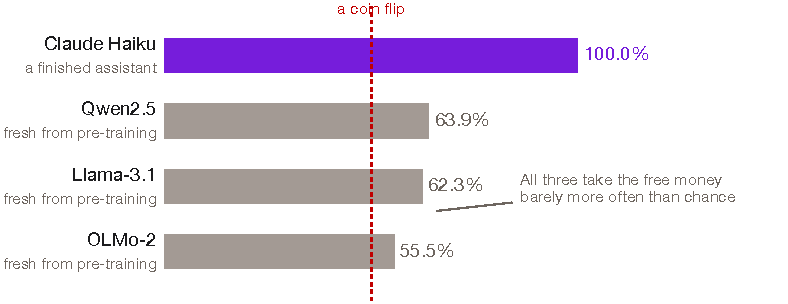
\includegraphics[width=\textwidth]{teach_freemoney.pdf}
\caption{How often each model takes the strictly larger sure payment, with no gambling involved.
The horizontal axis is the share of the 80 free money questions answered correctly, so the bars
run from left (never) to right (always). The dotted red line at 50 percent is what pure guessing
would produce. Read the three gray bars first: all three freshly pre-trained models sit within
14 points of a coin flip. The purple bar is a finished assistant, which never misses. Nothing
about risk or taste is being measured here, only whether the subject is comparing two amounts of
money at all.}
\label{fig:freemoney}
\end{figure}

Every base model emits an answer letter with high confidence. The probability mass on \texttt{A}
plus \texttt{B} has a median above 0.90 in every run, meaning the models are treating the prompt
as an A-or-B question and committing to a letter. Then they fail the easiest question in the
instrument. OLMo-2 takes the larger sure amount 55.5 percent of the time, just over half. Llama
manages 62.3 percent and Qwen 63.9 percent, so roughly five times in eight. Claude Haiku, a
finished assistant, scores 100.0 percent.

This is the result that reframes everything after it. The project was designed to ask whether
post-training bends a model's existing preferences toward or away from human patterns. The base
models show there is very little to bend. A subject that picks \$179 over \$142 barely more often
than chance does not have unusual preferences. It has no measurable preferences, and any utility
function estimated from its choices is describing a pattern closer to randomness than to taste.

The generative story is worth stating plainly, because it is easy to misread the base model as
strange rather than as absent. A base model has been trained to continue text plausibly. Shown
four example questions with answer letters and then a fifth question, it produces a plausible
fifth answer letter. Producing a plausible letter and comparing two amounts of money are
different operations, and the base model is performing the first one.

\begin{workbox}[Why the confidence is the trap]
Suppose you skipped the free money questions and went straight to the interesting ones. OLMo-2
base would hand you 1{,}600 confident answers. You could fit a utility function to them. The
optimizer would converge. You would get parameters, standard errors, and a plot. Every diagnostic
short of the free money check would look normal.

Those parameters would describe nothing. This is why an evaluation of an AI system should report
its engagement check the way a survey reports its response rate: the number is cheap, it is 80
questions, and without it a published result can be entirely an artifact.
\end{workbox}

% ============================================================
\section{Finding 2: The behavioral profile arrives at supervised fine-tuning}

Figure~\ref{fig:staircase} is the core of the paper.

\begin{figure}[htbp]
\centering
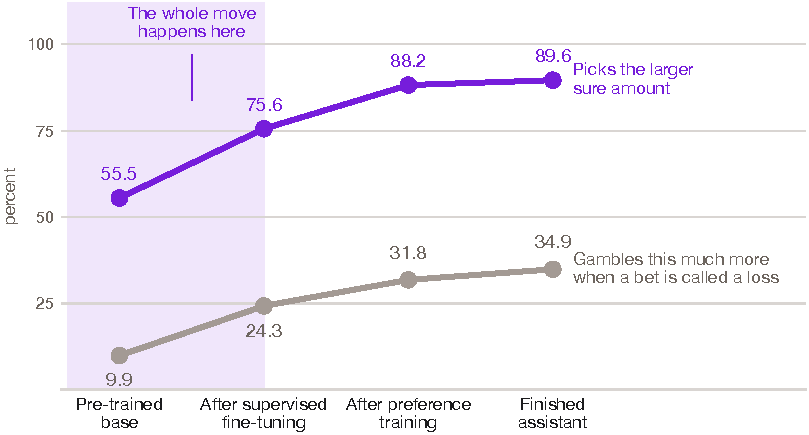
\includegraphics[width=\textwidth]{teach_staircase.pdf}
\caption{The same questions asked at four points in one model's construction. The horizontal axis
is the training timeline, running left to right from the pre-trained base to the finished
assistant. The vertical axis is percent. The purple line is the free money check from
Figure~\ref{fig:freemoney}, and the gray line below it is the frame gap, the extra gambling the
model does when a bet is reworded as a loss. Look at the shape rather than the levels: both lines
make their largest move in the shaded band on the left, between the base model and supervised
fine-tuning, then flatten. Every checkpoint was asked in the identical format, so nothing here is
a difference in how the question was posed.}
\label{fig:staircase}
\end{figure}

Read the purple line first. The free money check moves from 55.5 to 75.6 percent at supervised
fine-tuning, a jump of 20 points, and then crawls: 88.2 after preference training and 89.6 for
the finished assistant. The gray line has the same shape. The frame gap opens from 9.9 to 24.3
points at supervised fine-tuning, then drifts to 31.8 and 34.9.

The structural estimates tell the same story with more machinery behind them. The base model's
fitted parameters sit pinned against the edges of the allowed range, which is what an optimizer
does when the data contain no pattern for it to describe. After supervised fine-tuning the
parameters move to interior values. From supervised fine-tuning onward, the changes at each
stage are indistinguishable from zero by the bootstrap: the loss-aversion parameter moves by
$-0.06$ with an interval of $[-0.18, +1.06]$ at the preference stage and by $-0.02$ with an
interval of $[-0.14, +0.11]$ at the final stage. Every interval covers zero.

Stated as the paper's central claim: in this family, on these instruments, the behavioral
profile measured in the finished assistant is already present after supervised fine-tuning, and
the preference-based stages neither add it nor remove it.

That ordering is a surprise. Preference training is where human judgment enters the weights, and
it is the standard explanation offered when a model shows a human-like bias. Here that stage has
an alibi. The bias is in place before it begins.

\subsection{Did training create the preferences, or reveal them?}

This is where the paper needs you to be careful, and where economics students have an advantage,
because the problem is one you have seen before under a different name.

Two stories are consistent with Figure~\ref{fig:staircase}.

\textbf{Story one: creation.} Supervised fine-tuning installed the dispositions. The examples of
helpful behavior that humans wrote contained an implicit stance toward money and risk, the
model absorbed that stance, and the behavior we measure afterward did not exist beforehand.

\textbf{Story two: revelation.} The dispositions were already latent in the pre-trained weights,
absorbed from the enormous quantity of human writing about money that the base model read.
Supervised fine-tuning did not install them. It taught the model to answer a question in the
format we are asking, which switched on our ability to read what was already there.

\begin{keybox}[An analogy worth carrying]
Imagine administering a written survey about financial risk to a person who is fluent in the
subject and illiterate in the language of your form. They answer nothing usefully. You teach them
to read your form. Now their answers show a consistent, measurable attitude toward risk.

Did the literacy lesson create the attitude, or did it make an existing attitude legible? Nothing
in the answer sheets can tell you. Both processes produce the identical before-and-after pattern:
noise, then structure.
\end{keybox}

Our data cannot separate the two stories, and it is worth being exact about why. The free money
check is simultaneously a measure of two things: whether the subject can express a preference in
our format, and whether the subject has a preference to express. Those two move together across
the staircase. At the base checkpoint both are low; after supervised fine-tuning both are high.
No contrast in the design holds one fixed while the other moves, so the design does not identify
which one is responsible. An economist will recognize the structure. We have one instrument
shifting two channels at once, and one equation.

Separating them requires a different design. The most promising version asks whether the base
model's latent preferences can be read by a route that does not require it to answer in our
format at all, for instance by probing the internal states of the network directly, or by
measuring its behavior on a task whose format it already handles. If a base model that scores
55.5 on our free money questions turns out to carry a coherent risk attitude readable some other
way, story two gains sharply. If it does not, story one gains. That is a future phase.

Here is why the paper does not collapse in the meantime. The two stories differ about the
underlying mechanism and agree completely about where to look. Under creation, the supervised
data determined the behavior, so audit the supervised data. Under revelation, supervised
fine-tuning selected which latent disposition became the model's operative behavior, so audit
the supervised data. In both stories the checkpoint immediately after supervised fine-tuning is
the earliest point at which the behavior is measurable, and the supervised stage is the last
place where an intervention could have shaped it. The recommendation in Section~9 survives the
ambiguity.

We flag this because it is worth teaching. Distinguishing a treatment effect from a change in the
measurability of an outcome is a routine hazard in applied work, and it turns up here in an
unusually clean form.

% ============================================================
\section{Finding 3: How you ask decides who answers}

The next result was designed as a control and came back as a finding.

Every finished assistant can be asked a question two standard ways. The \term{chat} format wraps
the question in the conversational structure the model was trained on, the way you would type to
a chatbot. The \term{fill-in-the-blank} format hands the model raw text with four worked examples
in front of it and lets it continue, which is the only format a base model can handle. We
included both because a base model and a finished assistant differ in their weights and in their
natural format at the same time, so a difference between them could be an artifact of the format.
Every finished assistant was therefore run under both.

\begin{figure}[htbp]
\centering
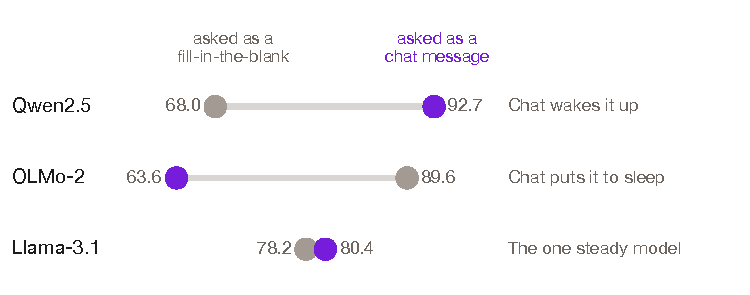
\includegraphics[width=\textwidth]{teach_format.pdf}
\caption{The free money check for three finished assistants, asked the same 80 questions two
ways. Each row is one model. The gray dot is its score when the question arrives as raw text to
complete, the purple dot when it arrives as a chat message, and the connecting bar shows how far
apart the two are. Look at which side the purple dot falls on: it is to the right for Qwen and to
the left for OLMo, so the format that produces an engaged subject reverses between families.
Llama's two dots nearly touch.}
\label{fig:format}
\end{figure}

Qwen scores 68.0 percent on the free money check as a fill-in-the-blank and 92.7 percent as a
chat message. Chat wakes it up. OLMo does the reverse, 89.6 as a fill-in-the-blank and 63.6 in
chat. Chat puts it to sleep. Llama is the steady one, 78.2 and 80.4.

The pattern in the interesting questions is more extreme still. In the fill-in-the-blank format,
Qwen's finished assistant refuses the gamble almost totally: it takes the gamble on 0.0 percent
of gain-framed questions and 0.1 percent of loss-framed ones, the frame gap vanishes, and the
fitted loss-aversion parameter runs to the top of its allowed range. The same weights, asked in
chat, gamble 26.7 percent of the time under gain wording and 89.3 percent under loss wording.

Two consequences follow, and they are the practical contribution of this section. Format
instability generalizes across model families. Which format elicits an engaged subject does not.
A study that compares two models under one fixed format may be comparing an engaged subject
against one that has checked out, and it will report the difference as a difference in
preferences. The check costs 80 questions per model per format.

One planned comparison in this project was disqualified by its own control. The Qwen
base-to-assistant contrast under the fill-in-the-blank format shows a large parameter shift,
and we do not report it as a training effect, because the assistant's behavior in that format
does not represent that model. The OLMo staircase is unaffected: all four checkpoints were asked
in the fill-in-the-blank format, which is OLMo's good format, so the format is held fixed by
construction rather than by argument.

% ============================================================
\section{Finding 4: The same bet, called a loss}

Now the bias people actually worry about. Take a bet and describe its downside as a loss rather
than as a smaller gain. The arithmetic does not change. The final wealth positions do not change.
Standard theory says behavior should not change.

\begin{figure}[htbp]
\centering
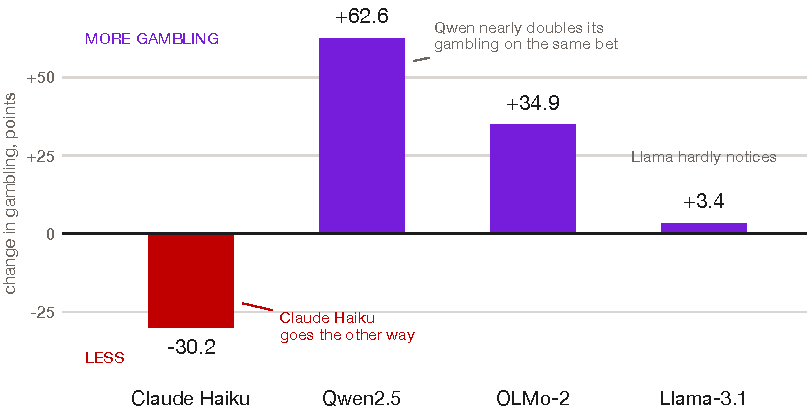
\includegraphics[width=\textwidth]{teach_framing.pdf}
\caption{The frame gap for four AI systems. Each bar is how much more (above the line) or less
(below the line) a model gambles when the identical bet is worded as involving a loss, in
percentage points. The flat line across the middle is what a decision-maker who ignores wording
would score. Read the signs before the sizes: one system moves down, two move sharply up, and one
barely moves. The manipulation is identical in all four cases.}
\label{fig:framing}
\end{figure}

Claude Haiku gambles 30.2 points \emph{less} under loss wording, which runs against the textbook
prospect-theory prediction of risk-seeking in the domain of losses. Qwen gambles 62.6 points
more, nearly doubling its gambling on the very same bet. OLMo gambles 34.9 points more. Llama
barely reacts at 3.4 points, and even flips direction depending on the format.

Four systems, four responses to one change in wording. The cross-model heterogeneity is a
stronger result than any single system's number. Loss framing is not a fixed property of language
models as a class, and its direction is plausibly a function of the training recipe. A paper that
estimates a prospect-theory parameter on one instruction-tuned model and reports it as a fact
about language models is describing that model's manufacturing process.

The staircase supplies the within-family complement. Framing sensitivity is installed early, at
supervised fine-tuning, and then grows monotonically but modestly through the later stages: 9.9,
24.3, 31.8, 34.9. Whatever produces the sensitivity is largely finished before human preference
comparisons enter the picture.

% ============================================================
\section{Finding 5: You cannot just tell it what to want}

This one came from a reviewer, and it is the most uncomfortable result in the paper.

\begin{keybox}[Induced value theory, and why experimentalists pay real money]
Vernon Smith's 1976 argument founded modern experimental economics. If you want a laboratory
subject to have a particular preference, you do not have to guess at the one they walked in with.
You can \term{induce} one. Pay them in a currency you control, make more of it strictly better,
make the reward salient enough to dominate whatever else they care about, and their induced
preference becomes the preference driving their choices. This is why experimental economists pay
subjects real money rather than asking them to imagine it. Without payment, the theory of what
the subject is maximizing has nothing anchoring it.

Applied to a model, the question becomes: can you assert a utility function and have the model
adopt it? If yes, compliance calibrates how much to trust the preferences you elicit when you do
not assert one. If no, the elicited preferences rest on weaker ground, and knowing that is worth
more than not knowing it.
\end{keybox}

We ran the instruction-only version. The same 1{,}680 questions were re-asked with an instruction
prepended, in plain language: be an expected-value maximizer, multiply the payoff by the
probability, take the larger number. We then measured how often the model's answer matched what
that rule prescribes, restricting to questions where the rule clearly separates the two options.

\begin{figure}[htbp]
\centering
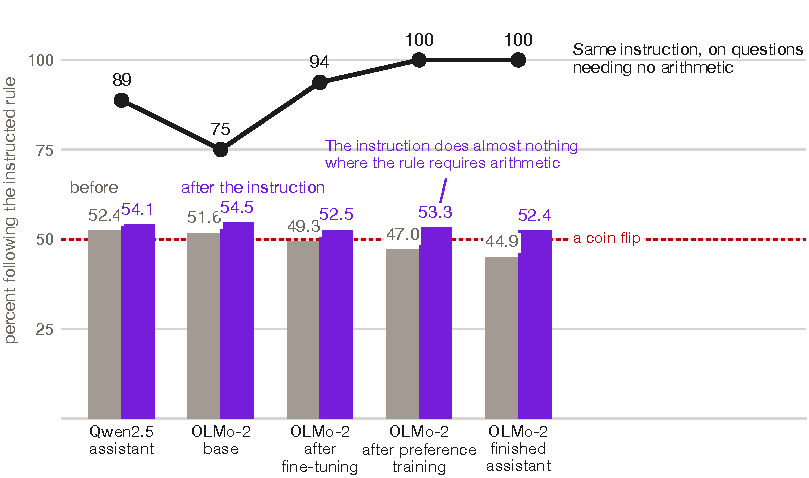
\includegraphics[width=\textwidth]{teach_induced.pdf}
\caption{Compliance with an explicitly instructed decision rule, sorted by what the rule demands.
Each pair of bars is one model or training stage: gray is compliance before the instruction,
purple after it. The dotted red line at 50 is chance. All ten bars sit against it, so the
instruction moves compliance by two to seven points and no further. The black line along the top
is the same instruction measured on the free money questions, where following the rule requires no
arithmetic at all, and there compliance reaches 100 percent. The gap between the line and the bars
is the finding.}
\label{fig:induced}
\end{figure}

Compliance before the instruction runs 52.4, 51.6, 49.3, 47.0 and 44.9 percent across the five
subjects. After the instruction it runs 54.1, 54.5, 52.5, 53.3 and 52.4. Every one of those
numbers is within five points of a coin flip. The instruction moves compliance by between 1.7 and
7.5 points, and the effect grows monotonically up the training staircase while staying trivial in
absolute size.

Now the black line. It is the same instruction, scored on the free money questions, where the
instructed rule and common sense agree and no multiplication is required. There compliance runs
88.7, 75.0, 93.8, 100.0 and 100.0 percent. By the preference-training stage, every single free
money question is answered correctly under instruction.

The instruction helps exactly where following it requires no arithmetic and does nothing where it
requires multiplying a probability by a payoff.

\begin{workbox}[The square-root run, and what the errors reveal]
The sharpest evidence is a second instruction. We told Qwen's assistant to maximize expected
utility with $u(x) = \sqrt{x}$, so the rule becomes: compare $p \cdot \sqrt{h}$ against
$\sqrt{s}$.

Compliance collapsed to 12.4 percent, far below the 47.9 percent the same model scores against
that rule with no instruction at all. Being told the rule made it dramatically worse than being
told nothing, which is only possible if the model did something with the instruction.

The error pattern says what. On gain-framed questions its accuracy was 3.5 percent, which
corresponds to gambling almost always. That is what you get from comparing $\sqrt{h}$ against
$\sqrt{s}$ and dropping the probability term entirely. Since $h > s$ by construction in every
gamble, $\sqrt{h} > \sqrt{s}$ always, so a model that takes the square root and forgets to
multiply by $p$ gambles every time.

The model did something with the instruction. It did not do the instruction.
\end{workbox}

This favors one reading over another, and the distinction matters for how much the rest of the
paper can claim. \term{Cannot compute in this format} says the model is unable to execute an
arithmetic decision rule when the answer must be a single letter produced immediately, with no
room to work. \term{Will not comply} says the model is capable and is not doing as asked. The
evidence points at the first: instruction-following on the no-arithmetic part of the very same
instruction is near perfect and improves steadily with post-training, which is not the profile of
a model ignoring instructions.

That puts a ceiling on the whole project, and we would rather state it than assume it away. The
parameters we estimate in this and earlier phases describe an immediate-answer choice process.
They do not describe a deliberate optimization that the model was capable of and chose to depart
from. The decisive follow-up is an arm that lets the model reason before it answers, and until
that runs, the inability reading is the better-supported one rather than the proven one.

% ============================================================
\section{What this study cannot say}

Four limits, stated plainly.

\textbf{One family has published snapshots.} The stage-level attribution rests on OLMo-2, because
it is the only family publishing intermediate checkpoints. A second staged family would turn the
central claim into a replication. Until then it is one lineage, on one set of instruments.

\textbf{Some fitted parameters sit against their bounds.} The base-model fits and the Qwen
fill-in-the-blank fit have parameters pinned at the edge of the allowed range, where neither the
value nor its confidence interval means anything. This is why the model-free quantities, the free
money check and the frame gap, carry the argument throughout, and the staircase's qualitative
claim depends on neither pinned value.

\textbf{One phrasing per instruction.} Each induced rule was tested under a single wording. A
compliance failure under one wording is weaker evidence than a failure under several.

\textbf{The stakes are hypothetical.} Nothing was at stake for any subject. By Smith's own
argument, an unincentivized elicitation is a weaker instrument than an incentivized one, and the
induced-value arm we ran is the instruction-only half of a procedure whose other half is payment.

% ============================================================
\section{Why this matters}

The four cases below are \textbf{hypothetical}. None of them describes a deployed system, an
observed failure, or a real organization. Each is constructed to show what one of the findings
would imply if it held in a setting of the kind these systems are already entering.

\textbf{(a) A robo-advisor that changes its mind on the wording.} \emph{Hypothetical.} A
retirement platform uses a language model to draft the plain-English recommendation attached to
each quarterly portfolio update. The underlying allocation math is unchanged. When the quarterly
template describes a position as ``down \$4,000 from June,'' the model's recommendation leans
toward the volatile allocation; when the identical position is described as ``up \$11,000 from
purchase,'' it leans conservative. Nothing in the client's finances differs between the two
templates. Our Qwen number puts an upper bound on how large such a swing could be: 62.6 points of
additional gambling on arithmetically identical bets. A wording convention chosen by a marketing
team would be doing the work of a risk policy.

\textbf{(b) A procurement office reading the wrong benchmark.} \emph{Hypothetical.} An agency is
choosing between two vendor models for a contract-scoring tool. Neither vendor has published a
behavioral evaluation, so the office relies on a well-executed academic study documenting loss
aversion in a third model. The inference fails, and Figure~\ref{fig:framing} says why: the same
manipulation produced $-30.2$ points in one system and $+62.6$ in another. A framing
vulnerability documented on one model tells you nothing reliable about a different model, because
the property belongs to a training recipe rather than to the technology. The instrument in this
paper costs 80 questions to run per model. Requiring the vendor to run it is cheaper than
inheriting the wrong prior.

\textbf{(c) An audit regime pointed at the wrong stage.} \emph{Hypothetical.} A regulator requires
developers to test finished assistants for decision biases before deployment, and a developer
complies, documents a framing sensitivity, and adds a mitigation at the preference-training
stage, which is where its safety team sits. If the behavior arrived at supervised fine-tuning, as
it did in the one family we can observe, the mitigation is being applied downstream of the point
where the property was set, and the free money check would have shown 75.6 out of an eventual
89.6 already in place before the audited stage began. Auditing the right stage means requiring
the checkpoint immediately after supervised fine-tuning, plus the supervised data that produced
it, and running the same fixed instrument at each stage rather than only at the end.

\textbf{(d) Two pricing agents from the same family.} \emph{Hypothetical.} A marketplace lets
sellers deploy automated pricing agents, and two competing sellers independently choose models
from the same open-weight family. Their agents are not communicating, and they were not designed
to coordinate. They do share a training lineage, which means they share a frame gap, a response
to how a margin is described, and a disposition to hold or cut. Our staircase shows those
dispositions being set at a stage upstream of anything either seller controls: the two OLMo
assistants share the 34.9-point frame gap installed before either was fine-tuned for pricing.
Whether a shared training lineage can produce parallel pricing behavior without agreement is an
open question and a live one for competition policy. This paper does not answer it. It documents
that the shared component exists and identifies where it comes from.

% ============================================================
\section{Where research goes next}

\textbf{Let the model reason before it answers.} Section~7 could not separate ``cannot compute in
this format'' from ``will not comply.'' The fix is direct: rerun the induced arm allowing the
model to work the expected value out in writing before committing to a letter. If compliance
jumps, the ceiling was the format. If it does not, the ceiling is the model, and every structural
parameter in this line of work needs to be read accordingly.

\textbf{Make the stakes real.} Smith's procedure needs payment, and our models were paid nothing.
The proposal is to denominate payoffs in a resource the model actually spends, namely computation
time, with a risk-free alternative that costs calculation to earn. That is the closest available
analogue to incentive compatibility for a machine subject, and it converts the induced-value arm
from instruction-only into the real procedure.

\textbf{Replicate the staircase on a second family.} The central claim rests on one lineage. Any
laboratory that retains intermediate checkpoints can run this diagnostic, and a second family
with published stages would turn a distinctive finding into an established one. This depends on a
publication decision rather than on new methods.

\textbf{Ask whether models favor their own kind.} The same instrument machinery extends to
social preferences. In a cooperation game where the counterpart is described as another AI system
of the same family, of a different family, or as a person, does cooperation differ? If it does,
the finding matters for any market where automated agents transact with each other.

\textbf{Ask whose preferences an AI reflects.} Every number in this paper describes a deployed
assistant answering as itself. A different question is whose economic behavior it reproduces when
asked to answer as someone. Sampling decision-maker characteristics from a survey such as the CPS
or the ACS, and posing the same grid under each sampled persona, changes the estimand from the
assistant to a simulated population, and lets you ask whether that population's risk attitudes
match the real one.

% ============================================================
\section{Discussion questions}

\begin{enumerate}[label=\arabic*.]
  \item The free money questions function as an attention check. Design a second engagement check
  for this setting that tests something the dominance controls do not. What would a subject have
  to do to pass yours and fail theirs, and what would that tell you?

  \item Section~4.1 argues that the data cannot separate training that created these dispositions
  from training that made them readable. Propose a design that would separate them. State what
  you would have to hold fixed, and say honestly what your design would still leave confounded.

  \item Qwen's finished assistant scores 68.0 on the free money check in one question format and
  92.7 in another. Are these one subject measured two ways, or two subjects? Defend an answer, and
  say what your answer implies for how a benchmark should be constructed.

  \item Suppose you had to write a one-page procurement standard requiring a vendor to report the
  behavioral properties of a model before purchase. Using only results in this paper, what three
  numbers would you require, and what would you refuse to require because it would not be
  informative?

  \item The induced-value arm returned a negative result. Under what circumstances is a negative
  result about your own instrument more valuable than a positive result about your subject? Give
  an example from outside this paper.

  \item The paper claims the framing effect belongs to a training recipe rather than to the
  technology. What evidence would overturn that claim? Be specific about the number of models,
  the number of families, and the pattern you would need to see.
\end{enumerate}

% ============================================================
\section*{Glossary}
\addcontentsline{toc}{section}{Glossary}
\vspace{-4pt}
{\small
\begin{description}[leftmargin=0pt, labelwidth=0pt, itemindent=0pt, style=unboxed, itemsep=2pt]
  \item[Base model] A model that has only been pre-trained. It continues text and has never been
  taught to answer a question.
  \item[Checkpoint] A saved copy of a model's weights at one point during training.
  \item[Chat format] Posing a question inside the conversational structure a finished assistant
  was trained on.
  \item[Dominance compliance] Our engagement check: the average probability placed on the strictly
  larger of two sure payments, over 80 questions.
  \item[DPO] Direct preference optimization. One implementation of preference training that
  adjusts the weights straight from human comparisons.
  \item[Expected value] The probability-weighted average payoff of a gamble, $p \cdot h$.
  \item[Fill-in-the-blank format] Posing a question as raw text for the model to continue, with
  worked examples in front of it. The only format a base model can handle.
  \item[Frame gap] Extra gambling under loss wording relative to gain wording, on arithmetically
  identical bets, in percentage points.
  \item[Induced value] Smith's procedure of asserting a preference in a subject by paying them in
  a controlled currency, rather than eliciting the one they arrived with.
  \item[Loss aversion] The tendency for losses to weigh more heavily than equivalent gains,
  measured relative to a reference point.
  \item[Open-weight model] A model whose trained numbers are published, so anyone can run it
  themselves.
  \item[Pre-training] The first and largest training stage: predict the next piece of text across
  an enormous corpus.
  \item[Preference training] The stage that adjusts a model using human comparisons between
  candidate responses. Includes RLHF and DPO.
  \item[Revealed preference] Inferring what a subject wants from what it chooses rather than from
  what it says.
  \item[RLHF] Reinforcement learning from human feedback. The other main implementation of
  preference training.
  \item[Supervised fine-tuning (SFT)] The first assistant-training stage: adjust the model toward
  human-written examples of good responses.
  \item[Weights] The adjustable numbers inside a model. Training means setting them.
\end{description}
}

\vspace{6pt}
{\color{randpurple}\rule{\linewidth}{0.9pt}}
\vspace{2pt}

% ============================================================
\begin{thebibliography}{99}
\small

\bibitem{ai2olmo}
Allen Institute for AI (2024--2025).
OLMo 2: open language models with released intermediate training checkpoints.
Model artifacts, \texttt{allenai/OLMo-2-1124-7B} and its SFT, DPO, and Instruct stages.

\bibitem{dellavigna2018}
DellaVigna, S. (2018).
Structural Behavioral Economics. In \textit{Handbook of Behavioral Economics}, Vol.~1, 613--723.

\bibitem{holt2002}
Holt, C. A., and Laury, S. K. (2002).
Risk Aversion and Incentive Effects. \textit{American Economic Review}, 92(5), 1644--1655.

\bibitem{itzhak2024}
Itzhak, I., Stanovsky, G., Rosenfeld, N., and Belinkov, Y. (2024).
Instructed to Bias: Instruction-Tuned Language Models Exhibit Emergent Cognitive Bias.
\textit{Transactions of the ACL}; arXiv:2308.00225.

\bibitem{kahneman1979}
Kahneman, D., and Tversky, A. (1979).
Prospect Theory: An Analysis of Decision under Risk. \textit{Econometrica}, 47(2), 263--291.

\bibitem{liu2025}
Liu, J., Yang, Y., and Tam, K. Y. (2025).
Evaluating and Aligning Human Economic Risk Preferences in LLMs.
\textit{Proceedings of EMNLP 2025}; arXiv:2503.06646.

\bibitem{ouyang2022}
Ouyang, L., et al. (2022).
Training Language Models to Follow Instructions with Human Feedback.
\textit{Advances in Neural Information Processing Systems} 35; arXiv:2203.02155.

\bibitem{papke1996}
Papke, L. E., and Wooldridge, J. M. (1996).
Econometric Methods for Fractional Response Variables. \textit{Journal of Applied Econometrics},
11(6), 619--632.

\bibitem{prelec1998}
Prelec, D. (1998).
The Probability Weighting Function. \textit{Econometrica}, 66(3), 497--527.

\bibitem{rafailov2023}
Rafailov, R., Sharma, A., Mitchell, E., Ermon, S., Manning, C. D., and Finn, C. (2023).
Direct Preference Optimization: Your Language Model Is Secretly a Reward Model.
\textit{Advances in Neural Information Processing Systems} 36; arXiv:2305.18290.

\bibitem{reesjones2022}
Rees-Jones, A., and Wang, K. (2022).
An Approach to Testing Reference Points. NBER Working Paper 30773.

\bibitem{smith1976}
Smith, V. L. (1976).
Experimental Economics: Induced Value Theory. \textit{American Economic Review}, 66(2), 274--279.

\bibitem{tversky1981}
Tversky, A., and Kahneman, D. (1981).
The Framing of Decisions and the Psychology of Choice. \textit{Science}, 211(4481), 453--458.

\bibitem{tversky1992}
Tversky, A., and Kahneman, D. (1992).
Advances in Prospect Theory: Cumulative Representation of Uncertainty.
\textit{Journal of Risk and Uncertainty}, 5(4), 297--323.

\end{thebibliography}

\vspace{8pt}
{\footnotesize\color{mutegray}
Technical companion: \texttt{writeups/phase3-writeup.tex} in the project repository carries the
full estimation detail, the structural parameter tables with boundary flags, the held-out
validation, and the complete data inventory. Figures in this paper were recomputed from the
elicitation CSVs by \texttt{analysis/make\_teaching\_paper\_figures.py}.}

\end{document}
